%!TEX root = da-dev.tex

In the previous chapter, we learned about the $\LOCAL$ model. We saw that with the help of unique identifiers, it is possible to gather the full information on a connected input graph in $O(\diam(G))$ rounds. To achieve this, we heavily abused the fact that we can send arbitrarily large messages. In this chapter we will see what can be done if we are only allowed to send small messages. With this restriction, we arrive at a model that is commonly known as the ``$\CONGEST$ model''.


\section{Definitions}\label{sec:congest}

Let $A$ be a distributed algorithm that solves a problem $\Pi$ on graph family $\calF$ in the $\LOCAL$ model. Assume that $\Msg_A$ is a countable set; without loss of generality, we can then assume that
\[
    \Msg_A = \NN,
\]
that is, the messages are encoded as natural numbers. Now we say that $A$ solves problem $\Pi$ on graph family $\calF$ in the $\CONGEST$ model if the following holds for some constant $C$: for any graph $G = (V,E) \in \calF$, algorithm $A$ only sends messages from set $\{0, 1, \dotsc, |V|^C\}$.

Put otherwise, we have the following \emph{bandwidth restriction}: in each communication round, along each edge, we can only send $O(\log n)$-bit messages, where $n$ is the total number of nodes.


\section{Examples}

Assume that we have an algorithm $A$ that was designed for the $\LOCAL$ model. Moreover, assume that during the execution of $A$ on a graph $G = (V,E)$, we only needs to send the following pieces of information along each edge:
\begin{itemize}[noitemsep]
    \item $O(1)$ node identifiers.
    \item $O(1)$ edges, encoded as a pair of node identifiers.
    \item $O(1)$ counters that take values from $0$ to $\diam(G)$.
    \item $O(1)$ counters that take values from $0$ to $|V|$.
    \item $O(1)$ counters that take values from $0$ to $|E|$.
\end{itemize}
Now it is easy to see that we can encode all of this as a binary string with $O(\log n)$ bits. Hence $A$ is not just an algorithm for the $\LOCAL$ model, but it is also an algorithm for the $\CONGEST$ model.

Many algorithms that we have encountered in this book so far are also $\CONGEST$ algorithms; we did not need to abuse large messages (see Exercise~\ref{ex:congest-prior}). However, there is a notable exception: algorithm $\algo{Gather}$ from Section~\ref{sec:gather}. In this algorithm, we may need to send up to $\Theta(n^2)$ bits of information along an edge:
\begin{itemize}
    \item To encode the set of nodes, we may need up to $\Theta(n \log n)$ bits. For example, we can encode it as a list of $n$ identifiers, each of which is $\Theta(\log n)$ bits long.
    \item To encode the set of edges, we may need up to $\Theta(n^2)$ bits. For example, we can give the adjacency matrix.
\end{itemize}
Of course we can write an algorithm that sends arbitrarily long bit strings in the $\CONGEST$ model, too, but this will take several communication rounds.

While algorithms with a running time of $O(\diam(G))$ or $O(n)$ are trivial in the $\LOCAL$ model, this is no longer the case in the $\CONGEST$ model. Indeed, there graph problems that \emph{cannot} be solved in time $O(n)$ in the $\CONGEST$ model.

In this chapter, we will learn techniques that can be used to design efficient algorithms in the $\CONGEST$ model. We will use the all-pairs shortest path problem as a running example.


\section{All-Pairs Shortest Path Problem}

Throughout this chapter, we will assume that the input graph $G = (V,E)$ is connected. In the \emph{all-pairs shortest path} problem (APSP in brief), the goal is to find the distances between all pairs of nodes. More precisely, the local output of node $v \in V$ is
\[
    f(v) = \bigl\{ (u, d) : u \in V,\ d = \dist_G(v, u) \bigr\}.
\]
That is, $v$ has to know the identities of all other nodes, as well as the shortest-path distance between itself and all other nodes.

Note that just to represent $f(v)$ we need $\Theta(n \log n)$ bits, and just to transmit this information along a single edge we would need $\Theta(n)$ communication rounds. Indeed, it is possible to prove that any algorithm that solves the APSP problem in the $\CONGEST$ will need $\Omega(n)$ rounds model\mydash see Exercise~\ref{ex:apsp-lb}.

In this chapter, we will present an optimal distributed algorithm for the APSP problem: it solves the problem in any connected graph in $O(n)$ rounds.

\newcommand{\BFS}{\algo{BFS}}
\newcommand{\Wave}{\algo{Wave}}

\longsection{Algorithm \talgo{Wave}}{Single-Source Shortest Paths}\label{sec:wave}

As a warm-up, we will start with a much simpler problem. Assume that we have elected a leader $s \in V$, that is, we have an input in which precisely one node, $s$, is labelled with $1$ and all other nodes are labelled with $0$. We will design an algorithm such that each node $v \in V$ outputs
\[
    f(v) = \dist_G(s,v),
\]
that is, its shortest-path distance to leader $s$. This is very simple. Initially, each node is in state $\bot$. In the first round, the leader will send message \msg{wave} to all neighbours and switch to state $0$ and stop. In round $i$, each node $v$ proceeds as follows: if $v$ has not stopped, and if it receives message \msg{wave} from some ports, it will send message \msg{wave} to all other ports, and then switch to state $i$ and stop. See Figure~\ref{fig:wave}.

\begin{figure}
    \centering
    \includegraphics[page=\PWave]{figs.pdf}
    \caption{(a)~Graph $G$ and leader~$s$. (b)~Execution of algorithm $\Wave$ on graph $G$. The arrows denote \msg{wave} messages, and the dotted lines indicate the communication round during which these messages were sent.}\label{fig:wave}
\end{figure}

The analysis of the algorithm is simple. By induction, all nodes at distance $i$ from $s$ will receive message \msg{wave} from at least one port in round $i$, and they will hence output the correct value~$i$. The running time of the algorithm is $O(\diam(G))$ rounds in the $\CONGEST$ model.


\longsection{Algorithm \talgo{BFS}}{Breadth-First Search Tree}\label{sec:bfs}

Algorithm $\Wave$ finds the shortest-path distances from a single source $s$. Now we will do something slightly more demanding: calculate not just distances but also a tree that represents all shortest paths.

More precisely, our goal is to construct a \emph{breadth-first search tree} (BFS tree) $T$ rooted at $s$. This is a spanning subgraph $T = (V,E')$ of $G$ such that $T$ is a tree, and for each node $v \in V$, the shortest path from $s$ to $v$ in tree $T$ is also a shortest path from $s$ to $v$ in graph $G$. We will also label each node $v \in V$ with a \emph{distance label} $d(v)$, so that for each node $v \in V$ we have
\[
    d(v) = \dist_T(s,v) = \dist_G(s,v).
\]
See Figure~\ref{fig:bfs} for an illustration. We will interpret $T$ as a directed graph, so that each edge is of form $(u,v)$, where $d(u) > d(v)$, that is, the edges point towards the root~$s$.

\begin{figure}
    \centering
    \includegraphics[page=\PBFS]{figs.pdf}
    \caption{(a)~Graph $G$ and leader~$s$. (b)~BFS tree $T$ (arrows) and distance labels $d(v)$ (numbers).}\label{fig:bfs}
\end{figure}

There is a simple centralised algorithm that constructs the BFS tree and distance labels: breadth-first search. We start with an empty tree and unlabelled nodes. First we label the leader $s$ with $d(s) = 0$. Then in step $i = 0, 1, \dotsc$, we visit each node $u$ with distance label $d(u) = i$, and check each neighbour $v$ of $u$. If we have not labelled $v$ yet, we will label it with $d(v) = i+1$, and add the edge $(u,v)$ in the BFS tree. This way all nodes that are at distance $i$ from $s$ in $G$ will be labelled with distance label $i$, and they will also be at distance $i$ from $s$ in~$T$.

We can implement the same idea as a distributed algorithm in the CONGEST model. We will call this algorithm $\BFS$. In the algorithm, each node $v$ maintains the following variables:
\begin{itemize}
    \item $d(v)$: when the algorithm finishes, $d(v)$ will be the distance label of node $v$.
    \item $p(v)$: pointer to the parent of node $v$ in tree $T$ (port number).
    \item $C(v)$: the set of children of node $v$ in tree $T$ (port numbers).
    \item $a(v)$: acknowledgement, set to $1$ when the subtree rooted at $v$ has been constructed.
\end{itemize}
Here $a(v) = 1$ denotes a stopping state. When the algorithm stops, variables $d(v)$ will be distance labels, tree $T$ is encoded in variables $p(v)$ and $C(v)$, and all nodes will have $a(v) = 1$.

Initially, we set $d(v) \gets \bot$, $p(v) \gets \bot$, $C(v) \gets \bot$, and $a(v) \gets 0$ for each node $v$, except for the root which has $d(s) = 0$. We will grow tree $T$ from $s$ with simple two-round iterations:
\begin{itemize}
    \item Each node $v$ with $d(v) \ne \bot$ and $C(v) = \bot$ will send a \emph{proposal} with value $d(v)$ to all neighbours.
    \item If a node $u$ with $d(u) = \bot$ receives some proposals with value $j$, it will \emph{accept} one of them and \emph{reject} all other proposals. It will send $p(u)$ to point to the node whose proposal it accepted, and it will set $d(u) \gets j$.
    \item Each node $v$ that sent some proposals will set $C(v)$ to contain all neighbours that accepted proposals.
\end{itemize}
This way $T$ will grow towards the leaf nodes. Once we reach a leaf node, we will send acknowledgements back towards the root:
\begin{itemize}
    \item Each node $v$ with $a(v) = 0$ and $C(v) = \emptyset$ will set $a(v) \gets 1$.
    \item Each node $v$ with $a(v) = 1$ and $p(v) \ne \bot$ will send \emph{acknowledgements} to port $p(v)$.
    \item Each node $v$ with $a(v) = 0$ and $C(v) \ne \emptyset$ will set $a(v) \gets 1$ when it receives acknowledgements from each port of $C(v)$.
\end{itemize}
It is straightforward to verify that the algorithm indeed works and it constructs a BFS tree with distance labels in $O(\diam(G))$ rounds in the $\CONGEST$ model.

Note that the acknowledgements would not be strictly necessary in order to construct the tree. However, they will be very helpful in subsequent sections when we use algorithm $\BFS$ as a subroutine.


\longsection{Algorithm \talgo{Leader}}{Leader Election}\label{sec:leader}

Algorithm $\BFS$ constructs a BFS tree rooted at a single leader. Now we will show how to elect a leader. Surprisingly, we can use algorithm $\BFS$ here to \emph{elect} a leader, even if $\BFS$ \emph{assumes} that we have a leader!

We will design an algorithm $\algo{Leader}$ that finds the node with the smallest identifier; this node will be the leader. The basic idea is very simple:
\begin{enumerate}
    \item We modify algorithm $\BFS$ so that we can run multiple copies of it in parallel, with different root nodes. We augment messages with the identity of the root node, and each node keeps track of variables $d$, $p$, $C$, and $a$ separately for each possible root.
    \item Then we pretend that all nodes are leaders and start running $\BFS$. In essence, we will run $n$ copies of $\BFS$ in parallel, and hence we will construct $n$ BFS trees, one rooted at each node. We will denote with $\BFS_v$ the $\BFS$ process rooted at node $v \in V$, and we will write $T_v$ for the output of this process.
\end{enumerate}
However, there are two problems: First, it is not yet obvious how all this would help with leader election. Second, we cannot implement this idea directly in the $\CONGEST$ model\mydash nodes would need to send up to $n$ distinct messages per communication round, one per each $\BFS$ process, and there is not enough bandwidth for all those messages.

\begin{figure}
    \centering
    \includegraphics[page=\PLeader]{figs.pdf}
    \caption{Leader election. Each node $v$ will launch a process $\BFS_v$ that attempts to construct a BFS tree $T_v$ rooted at $v$. Other nodes will happily follow $\BFS_v$ if $v$ is the smallest leader they have seen so far; otherwise they will start to ignore messages related to $\BFS_v$. Eventually, precisely one of the processes will complete successfully, while all other process will get stuck at some point. In this example, here node $1$ will be the leader, as it has the smallest identifier. For example, process $\BFS_2$ will never succeed, as node $1$ (as well as all other nodes that are aware of node $1$) will ignore all messages related to $\BFS_2$. Node $1$ is the only root that will receive acknowledgements from every child.}\label{fig:leader}
\end{figure}

Fortunately, we can solve both of these issues very easily; see Figure~\ref{fig:leader}:
\begin{enumerate}[resume]
    \item Each node will only process and send messages related to the tree that has the \emph{smallest identifier as the root}. More precisely, for each node $v$, let $U(v) \subseteq V$ denote the set of nodes $u$ such that $v$ has received messages related to process $\BFS_u$, and let $\ell(v) = \min U(v)$ be the smallest of these nodes. Then $v$ will simply ignore messages related to process $\BFS_u$ for all $u \ne \ell(v)$, and it will only process and send messages related to process $\BFS_{\ell(v)}$.
\end{enumerate}
We make the following observations:
\begin{itemize}
    \item In each round, each node will only need to send messages related to at most one $\BFS$ process. Hence we have solved the second problem: now we can easily implement this algorithm in the $\CONGEST$ model.
    \item Let $s = \min V$ be the node with the smallest identifier. Then whenever process $\BFS_s$ reaches a node $v$, it will set $\ell(v) = s$ and never change it again. Hence all nodes will faithfully run $\BFS_s$ from start to end, and thanks to the acknowledgements, node $s$ will eventually know that we have successfully constructed a BFS tree $T_s$ rooted at it.
    \item Let $u \ne \min V$ be any other node. Now there is at least one node, $s$, that will ignore all messages related to process $\BFS_u$. Hence $\BFS_u$ will never finish; node $u$ will never receive acknowledgements related to tree $T_u$.
\end{itemize}
That is, we now have an algorithm with the following properties: after $O(\diam(G))$ rounds, there is precisely one node $s$ that knows that it is the unique node $s = \min V$. To finish the leader election process, node $s$ will simply use $T_s$ to inform all other nodes that leader election is over; node $s$ will output $1$ and all other nodes will output $0$ and stop.


\longsection{Algorithm \talgo{APSP}}{All-Pairs Shortest Paths}\label{sec:apsp}

In this section, we will design algorithm $\algo{APSP}$ that solves the all-pairs shortest path problem (APSP) in time $O(n)$.

We already know how to find the shortest-path distances from a single source; this is efficiently solved with algorithm $\Wave$. Just like we did with the $\BFS$ algorithm, we can also augment $\Wave$ with the root identifier and hence have a separate process $\Wave_v$ for each possible root $v \in V$. If we could run all these processes, then each node would receive a wave from every other node, letting us to solve the APSP problem. However, it is not obvious how to achieve a good performance in the $\CONGEST$ model:
\begin{itemize}
    \item If we try to run all $\Wave_v$ processes simultaneously in parallel, we may need to send messages related to several waves simultaneously along a single edge, and there is not enough bandwidth to do that.
    \item If we try to run all $\Wave_v$ processes sequentially, it will take a lot of time: the running time would be $O(n \diam(G))$ instead of $O(n)$.
\end{itemize}
The solution is to \emph{pipeline} the $\Wave_v$ processes so that we can have many of them running simultaneously in parallel, without congestion. In essence, we want to have multiple wavefronts active simultaneously so that they never collide with each other.

To achieve this, we start with the leader election and the construction of a BFS tree rooted at the leader; let $s$ be the leader, and let $T_s$ be the BFS tree. Then we do a \emph{depth-first traversal} of $T_s$. This is a walk $w_s$ in $T_s$ that starts at $s$, ends at $s$, and traverses each edge precisely twice; see Figure~\ref{fig:dfs}.

\begin{figure}
    \centering
    \includegraphics[page=\PDFS]{figs.pdf}
    \caption{(a)~BFS tree $T_s$ rooted at $s$. (b)~A depth-first traversal $w_s$ of $T_s$.}\label{fig:dfs}
\end{figure}

More concretely, we move a \emph{token} along walk $w_s$. Moreover, we move the token \emph{slowly}: we always spend 2 communication rounds before we move the token to an adjacent node. Whenever the token reaches a new node $v$ that we have not encountered previously during the walk, we launch process $\Wave_v$. This is the entire algorithm!

The key observation here is that the token moves slower than the waves. The waves move at speed $1$ edge per round, while the token moves at speed $0.5$ edges per round. This guarantees that two waves never collide. To see this, consider two waves $\Wave_u$ and $\Wave_v$, so that $\Wave_u$ was launched before $\Wave_v$. Let $d = \dist_G(u,v)$. Now it took us at least $2d$ rounds to move the token from $u$ to $v$, but only $d$ rounds for $\Wave_u$ to reach node $v$. Hence $\Wave_u$ was already past $v$ before we triggered $\Wave_v$, and $\Wave_v$ will never catch up with $\Wave_u$ as both travel at the same speed. See Figure~\ref{fig:pipeline} for an illustration.

\begin{figure}
    \centering
    \includegraphics[page=\PPipeline]{figs.pdf}
    \caption{Algorithm $\algo{APSP}$: the token walks along the BFS tree at speed $0.5$ (thick arrows), while each $\Wave_v$ moves along the original graph at speed $1$ (dashed lines). The waves are strictly nested: if $\Wave_v$ was triggered after $\Wave_u$, it will never collide with $\Wave_u$.}\label{fig:pipeline}
\end{figure}

Hence we have an algorithm $\algo{APSP}$ that is able to trigger all $\Wave_v$ processes in $O(n)$ time, without collisions, and each of them completes $O(\diam(G))$ rounds after it was launched. Overall, it takes $O(n)$ rounds for all nodes to learn distances to all other nodes. Already during $\algo{Leader}$ all nodes learned the identifiers of all other nodes, so we will also know when it is safe to stop: as soon as we have sent the token back towards the root and we have received all waves from all other nodes.


\section{Exercises}

\begin{ex}[prior algorithms]\label{ex:congest-prior}
    In Chapters \ref{ch:pn} and \ref{ch:local} we have seen examples of algorithms that were designed for the $\PN$ and $\LOCAL$ models. Many of these algorithms use only small messages\mydash they can be used directly in the $\CONGEST$ model. Give at least three examples of such algorithms.
\end{ex}

\begin{ex}[edge counting]
    The \emph{edge counting} problem is defined as follows: each node has to output the value $|E|$, i.e., it has to indicate how many edges there are in the graph.

    Assume that the input graph is connected. Design an algorithm that solves the edge counting problem in the $\CONGEST$ model in time $O(\diam(G))$.
\end{ex}

\begin{ex}[detecting bipartite graphs]
    Assume that the input graph is connected. Design an algorithm that solves the following problem in the $\CONGEST$ model in time $O(\diam(G))$:
    \begin{itemize}[noitemsep]
        \item If the input graph is bipartite, all nodes output $1$.
        \item Otherwise all nodes outputs $0$.
    \end{itemize}
\end{ex}

\begin{ex}[detecting complete graphs]
    We say that a graph $G = (V,E)$ is \emph{complete} if for all nodes $u, v \in V$, $u \ne v$, there is an edge $\{u,v\} \in E$.

    Assume that the input graph is connected. Design an algorithm that solves the following problem in the $\CONGEST$ model in time $O(1)$:
    \begin{itemize}[noitemsep]
        \item If the input graph is a complete graph, all nodes output $1$.
        \item Otherwise all nodes output $0$.
    \end{itemize}
\end{ex}

\begin{ex}[gathering]
    Assume that the input graph is connected. In Section~\ref{sec:gather} we saw how to gather full information on the input graph in time $O(\diam(G))$ in the $\LOCAL$ model. Design an algorithm that solves the problem in time $O(|E|)$ in the $\CONGEST$ model.
\end{ex}

\begin{exs}[gathering lower bounds]\label{ex:congest-gather-lb}
    Assume that the input graph is connected. Prove that there is no algorithm that gathers full information on the input graph in time $O(|V|)$ in the $\CONGEST$ model.

    \hint{To reach a contradiction, assume that $A$ is an algorithm that solves the problem. For each $n$, let $\calF(n)$ consists of all graphs with the following properties: there are $n$ nodes with unique identifiers $1,2,\dotsc,n$, the graph is connected, and the degree of node $1$ is $1$. Then compare the following two quantities as a function of~$n$:
    \begin{enumerate}
        \item $f(n) = {}$how many different graphs there are in family $\calF(n)$.
        \item $g(n) = {}$how many different message sequences node number $1$ may receive during the execution of algorithm~$A$ if we run it on any graph $G \in \calF(n)$.
    \end{enumerate}
    Argue that for a sufficiently large $n$, we will have $f(n) > g(n)$. Then there are at least two different graphs $G_1, G_2 \in \calF(n)$ such that node $1$ receives the same information when we run $A$ on either of these graphs.}
\end{exs}

\begin{exs}[APSP lower bounds]\label{ex:apsp-lb}
    Assume that the input graph is connected. Prove that there is no algorithm that solves the APSP problem in time $o(|V|)$ in the $\CONGEST$ model.
\end{exs}


\section{Bibliographic Notes}

The name $\CONGEST$ is from Peleg's~\cite{peleg00distributed} book. Algorithm $\algo{APSP}$ is due to Holzer and Wattenhofer \cite{holzer12apsp}\mydash surprisingly, it was published only as recently as in 2012.
